\section{Wyniki eksperymentów symulacyjnych}
\begin{frame}
\frametitle{\secname}
\framesubtitle{\textit{Otwarta przestrzeń prostopadłe} ustawienie: \textit{1-2}.}

\begin{textblock*}{0.4\paperwidth}(0.3\paperwidth,0.85cm)
	\begin{figure}[ht] % h:here; t:top; b:bottom; p:page; default:ht
		\centering
		\includegraphics[page = 2, width=0.4\paperwidth]{img/Simulation_Open_space.pdf}
\end{figure}
\end{textblock*}

\begin{textblock*}{\paperwidth}(0cm,5.45cm)
\begin{figure}[ht] % h:here; t:top; b:bottom; p:page; default:ht
	\captionsetup[subfigure]{labelformat=empty}
	\centering
	\subfloat[][R]
	{		
		\includemovie[autoplay,repeat]{0.235\paperwidth}{3cm}{mov/symulation/OtwartaPrzestrzenR1-2.mpg}
	}
	\subfloat[][RVO]
	{
		\includemovie[autoplay,repeat]{0.235\paperwidth}{3cm}{mov/symulation/OtwartaPrzestrzenR1-2.mpg}
	}
	\subfloat[][PR]
	{	
		\includemovie[autoplay,repeat]{0.235\paperwidth}{3cm}{mov/symulation/OtwartaPrzestrzenR1-2.mpg}
	}
	\subfloat[][R+]
	{
		\includemovie[autoplay,repeat]{0.235\paperwidth}{3cm}{mov/symulation/OtwartaPrzestrzenR1-2.mpg}
	}
\end{figure}
\end{textblock*}
\end{frame}